%-------------------------------------------------------------------------------
%	PACKAGES AND OTHER DOCUMENT CONFIGURATIONS
%-------------------------------------------------------------------------------
\documentclass[11pt,a4paper,english,twoside,onecolumn]{article}
\pagenumbering{arabic}
\usepackage{setspace}
%\onehalfspace
\usepackage[hmarginratio=1:1,top=32mm,columnsep=20pt]{geometry}
\usepackage{fancyhdr}
\usepackage{multirow}
\usepackage{multicol}
\usepackage[section]{placeins}
%---Text and Style--------------------------------------------------------------
\usepackage{microtype} 			% Slightly tweak font spacing for aesthetics
\usepackage[english]{babel}	% Language hyphenation and typographical rules
\usepackage[T1]{fontenc}
\usepackage[utf8]{inputenc}
\usepackage{ae}
\usepackage{relsize}
\usepackage{csquotes}
\usepackage{amsmath}
\usepackage{amsfonts}
\usepackage{mathdots}
\usepackage{mathtools}
\usepackage{ mathrsfs }
\usepackage[colorlinks=true]{hyperref}
\hypersetup{
	bookmarksnumbered=true,
	linkcolor=black,
	citecolor=black,
	urlcolor=black,
}
\usepackage{verbatim}
\usepackage{alltt}
\usepackage{lipsum}
\usepackage{siunitx}
\usepackage[inline]{enumitem}
\usepackage{lettrine}
\DeclareMathOperator{\sgn}{sgn}
\DeclareMathOperator{\RealNumber}{\rm I\!R}
\DeclarePairedDelimiter{\abs}{\lvert}{\rvert}
\DeclarePairedDelimiter{\norma}{\lVert}{\rVert}
%---Figure----------------------------------------------------------------------
\usepackage{graphicx}
\graphicspath{{./imgs/}}
\renewcommand{\figurename}{Fig.}
\usepackage{subfig}
%----Code-----------------------------------------------------------------------
\usepackage{algorithmicx}
\usepackage[ruled]{algorithm}
\usepackage{algpseudocode}
\usepackage{listings}
\usepackage{xcolor}
%---Table-----------------------------------------------------------------------
\usepackage{tabularx}
\usepackage{array}
\usepackage{color}
\usepackage{adjustbox}
\usepackage{colortbl}
\usepackage{pgfplotstable}
\usepackage{makecell}
\usepackage{booktabs}
%-------------------------------------------------------------------------------
% Allows abstract customization
\usepackage{abstract}
% Set the "Abstract" text to bold
\renewcommand{\abstractnamefont}{\normalfont\bfseries}
% Set the abstract itself to small italic text
\renewcommand{\abstracttextfont}{\normalfont\small\itshape}
% Allows customization of titles
\usepackage{titlesec}
% Roman numerals for the sections
\renewcommand\thesection{\Roman{section}}
% roman numerals for subsections
\renewcommand\thesubsection{\roman{subsection}}
\renewcommand\thesubsubsection{\alph{subsubsection}}
% Change the look of the section titles
\titleformat{\section}[block]{\Large\scshape\centering}{\thesection.}{1em}{}
% Change the look of the section titles
\titleformat{\subsection}[block]{\Large}{\thesubsection.}{1em}{}
\titleformat{\subsubsection}[block]{\large}{\thesubsubsection.}{1em}{}
\usepackage{titling} % Customizing the title section
%----Tikz-----------------------------------------------------------------------
\usepackage{tikz,fp,ifthen,fullpage}
\usepackage{pgfmath, pgfplots, xparse}
\usepackage{tikz-dimline, calc}
\usepgfplotslibrary{fillbetween}
\usetikzlibrary{backgrounds, arrows}
\usetikzlibrary{decorations.pathmorphing,fit,through}
\usetikzlibrary{shapes,decorations,shadows}
\usetikzlibrary{fadings,patterns,mindmap}
\pgfplotsset{compat=newest}

%-------------------------------------------------------------------------------
%	TITLE SECTION
%-------------------------------------------------------------------------------
\setlength{\droptitle}{-4\baselineskip} % Move the title up
\pretitle{\begin{center}\Huge\bfseries} % Article title formatting
\posttitle{\end{center}} 								% Article title closing formatting
\title{TITOLO DA INSERIRE} 							% Article title %TODO scegliere e inserire titolo
\author{%
	\textsc{Francesco Argentieri}\thanks{ID: 183892}\\[1ex] % Your name
	\normalsize Università di Trento \\ % Your institution
	% Your email address
	\normalsize \href{mailto:francesco.argentieri@studenti.unitn.it}{francesco.argentieri@studenti.unitn.it}
	}
\date{} % Leave empty to omit a date
%\renewcommand{\maketitlehookd}{\input{abstract}}
%-------------------------------------------------------------------------------
\begin{document}
	% Print the title
	\maketitle
	% Sommario Introduzione
	\section{Exercise 1}
\label{sec:problem}
The vibration absorber \cite{rao2011mechanical}[Ch. 9.11], also called dynamic vibration absorber, is
a mechanical device which is used to reduce or eliminate unwanted vibration.
It consists of a mass and a spring attached to the main (or original) mass that
needs to be protected from vibration. Vibration absorbers are commonly used in a
variety of applications which include sanders, saws, internal combustion engines
and high-voltage transmission lines. A sketch of the system is pictured in
Figure \ref{fig:system}.\linebreak

\begin{figure}[!h]
	\centering
	\begin{tikzpicture}[scale=0.85]
%	\draw[help lines] (0,0) grid [step = 5 mm](15,15);
%	\foreach \x in {0,1,...,15}
%	   \draw [help lines] (\x,0) node [below,%
%	          font=\footnotesize] {$\x$} -- (\x,0);
%	\foreach \y in {0,1,...,15}
%	   \draw [help lines] (0,\y) node [left,%
%	          font=\footnotesize] {$\y$} -- (0,\y);

	% Define style for spring
	\tikzstyle{springshape}=[decoration={aspect=0.6, segment length=1.5mm, amplitude=1mm, coil}, decorate];
	\newcommand{\spring}[3]{%
		% pass 3 arguments:
		% arg1: #1 coordinate x; arg2: #2 coordiante y; arg3: #3 number of componets
		\coordinate (attachleftside) at ({#1},{#2});
		\coordinate (startspring) at ($(attachleftside) + (0,0.25)$);
		\coordinate	(endspring) at ($(startspring) + (0,2)$);
		\coordinate	(attachrightside) at ($(endspring) + (0,0.25)$);
		\draw (attachleftside) -- (startspring);
		\draw [springshape] (startspring) -- (endspring) node[draw=none,pos=0.5, left] (){$\frac{k_{#3}}{2}$};
		\draw (endspring) -- (attachrightside);
	}

	\newcommand{\shortspring}[3]{%
		% pass 3 arguments:
		% arg1: #1 coordinate x; arg2: #2 coordiante y; arg3: #3 number of componets
		\coordinate (attachleftside) at ({#1},{#2});
		\coordinate (startspring) at ($(attachleftside) + (0,0.25)$);
		\coordinate	(endspring) at ($(startspring) + (0,1)$);
		\coordinate	(attachrightside) at ($(endspring) + (0,0.25)$);
		\draw (attachleftside) -- (startspring);
		\draw [springshape] (startspring) -- (endspring) node[draw=none,pos=0.5,left] (){$k_{#3}$};
		\draw (endspring) -- (attachrightside);
	}

	% Define style for dampers
	\tikzstyle{dampshape}=[decoration={markings, mark connection node=dmp,
	  mark=at position 0.5 with
	  {
	    \node (dmp) [inner sep=0pt,transform shape,rotate=-90,minimum width=15pt,minimum height=3pt,draw=none] {};
	    \draw  ($(dmp.north east)+(2pt,0)$) -- (dmp.south east) -- (dmp.south west) -- ($(dmp.north west)+(2pt,0)$);
	    \draw ($(dmp.north)+(0,-5pt)$) -- ($(dmp.north)+(0,5pt)$);
	  }
	}, decorate]
	\newcommand{\dampers}[3]{%
		% pass 3 arguments:
		% arg1: #1 coordinate x; arg2: #2 coordiante y; arg3: #3 number of componets
		\coordinate (attachleftside) at ({#1},{#2});
		\coordinate (startdamp) at ($(attachleftside) + (0,0.25)$);
		\coordinate	(enddamp) at ($(startdamp) + (0,1)$);
		\coordinate	(attachrightside) at ($(enddamp) + (0,0.25)$);
		\draw (attachleftside) -- (startdamp);
		\draw [{dampshape}] (startdamp) -- (enddamp) node[draw=none,pos=0.75, right] (){$c_{#3}$};
		\draw (enddamp) -- (attachrightside);
	}

	% Define ground
	\tikzstyle{ground}=[fill,pattern=north east lines,draw=none,minimum height=0.2cm];
	\tikzstyle{groundc}=[fill,pattern=north east lines,draw=none,minimum height=0.2cm];

	% generate plot
	\begin{scope}
		\draw (4,4.5) rectangle (11,7) node[draw=none,pos=0.5] () {Machine $m_{1}$};
		\draw (6.5,2.5) rectangle (8.5,1.5) node[draw=none,pos=0.5] () {$m_{2}$};
		\spring{5}{1}{1};
		\spring{10}{1}{1};
		\shortspring{7}{2.5}{2};
		\dampers{8}{2.5}{1};
		\draw (5,0) -- (5,1);
		\draw (5,3.5) -- (5,4.5);
		\draw  (10,0) -- (10,1);
		\draw (10,3.5) -- (10,4.5);
		\draw(7,4)--(7,4.5);
		\draw(8,4)--(8,4.5);
		\draw [groundc]  (4,0) rectangle (11,-0.2);
		\draw [dashed] (6.25,4.25) rectangle(8.75,1.25);
		\draw [-stealth] (7.5,7.5) -- (7.5,7)node[draw=none,pos=0.5, above right] () {$u$};
		\draw [-stealth] (11.5,5.75) -- (11.5,5.25)node[draw=none,pos=0.5, above right] () {$q_1$};
		\draw [-stealth] (9,2) -- (9,1.50)node[draw=none,pos=-0.25, above] () {$q_2$};
	\end{scope}
	\end{tikzpicture}
	\caption{Representation of the harmonic absorber.}
	\label{fig:system}
\end{figure}
\noindent The equations of motion for this two-degrees of freedom system can easily
obtained using a Lagrange formulation and can be conveniently written in the
following matrix form:
\begin{equation}
	\label{eq:matrixform}
	\begin{bmatrix}
		m_1 & 0 \\
		0 	&	m_2 \\
	\end{bmatrix}
	\begin{Bmatrix}
		\ddot{q_1}\\
		\ddot{q_2}\\
	\end{Bmatrix} +
	\begin{bmatrix}
		c_2 & -c_2 \\
		-c_2 	&	c_2 \\
	\end{bmatrix}
	\begin{Bmatrix}
		\dot{q_1}\\
		\dot{q_2}\\
	\end{Bmatrix}+
	\begin{bmatrix}
		k_1+k_2 & -k_2 \\
		-k_2 	&	k_2 \\
	\end{bmatrix}
	\begin{Bmatrix}
		q_1\\
		q_2\\
	\end{Bmatrix}
	=
	\begin{bmatrix}
		u \\
		0 \\
	\end{bmatrix}
\end{equation}


\section{Answer}
\subsection{1}
Starting from the equation of motion, seen in the equation \eqref{eq:matrixform},
we obtain the state space representation as below:
\[
	A =
	\begin{bmatrix}
		0  	& 		0 		&      1	 	&     0\\
		0 	&     0 		&      0 		&     1\\
		\frac{-(k_1 + k_2)}{m_1} & \frac{k_2}{m_1} & \frac{-c_2}{m_1} & \frac{c_2}{m_1}\\
		\frac{k_2}{m_2} & \frac{-k_2}{m_2} & \frac{c_2}{m_2} & \frac{-c_2}{m_2}
	\end{bmatrix}\quad
	B =
	\begin{bmatrix}
		0\\
		0\\
		\frac{1}{m_1}\\
		0
	\end{bmatrix}\quad
	C =
	\begin{bmatrix}
		1   &  0   &  0  &   0
	\end{bmatrix}
\]

\subsection{2}
Setting \(u\,=\,0\) through the help of the \emph{sdpt3} solver the solution
was solved numerically, obtaining the solution from the Lyapunov inequality for
 \(\mathbf{P}\) given in the matrix \eqref{eq:valuep} is obtained.
 \begin{equation}
 	\label{eq:valuep}
 	\begin{bmatrix*}[r]
 		603.3417	&   -8.5265	&    0.1252	&   -5.0157\\
		-8.5265	&  128.7847	&    2.8368	&    0.6276\\
		0.1252	&    2.8368	&    3.9082	&    0.5233\\
		-5.0157	&    0.6276	&    0.5233	&    1.1363
	\end{bmatrix*}
\end{equation}

\begin{equation}
	\label{eq:eigvalue}
	\begin{bmatrix*}[r]
		-0.7983 +14.2721i\\
  		-0.7983 -14.2721i\\
  		-0.3517 + 9.8873i\\
  		-0.3517 - 9.8873i\\
	\end{bmatrix*}
\end{equation}

\subsection{3}
Using the LMI formulation\cite{notelmi} and using the ``\emph{sdpt3}" solver the
 \(\mathcal{L}_{2}\) value of the \(\gamma\) system is estimated.
Where the minimum value assumed by \(\gamma\) is \num{0.5456e-3}.
Moreover, the same result was obtained using the matlab toolbox.

\subsection{4}
From the calculation of the transfer matrix \eqref{eq:tf}, calculated in, we
obtain the Bode diagram in the figure \ref{fig:bodeplot}, where we can see that
the peak has a value of \num{0.5440015e-03}.
\begin{align}
	\label{eq:tf}
	\begin{split}
		G(s) 	& = \frac{y(s)}{u(s)} = C(sI-A)^{-1}B\\
				& = \frac{0.01 s^2 + 0.02 s + 1.333}{s^4 + 2.3 s^3 + 303.3 s^2 + 300 s + 20000}
	\end{split}
\end{align}
It is observed that the value of \(\mathcal{L}_{2} = \num{0.5456e-3}\)  is
similar to the peak present in the Bode diagram in Figure \ref{fig:bodeplot}.
\begin{figure}[htb]
	\centering
	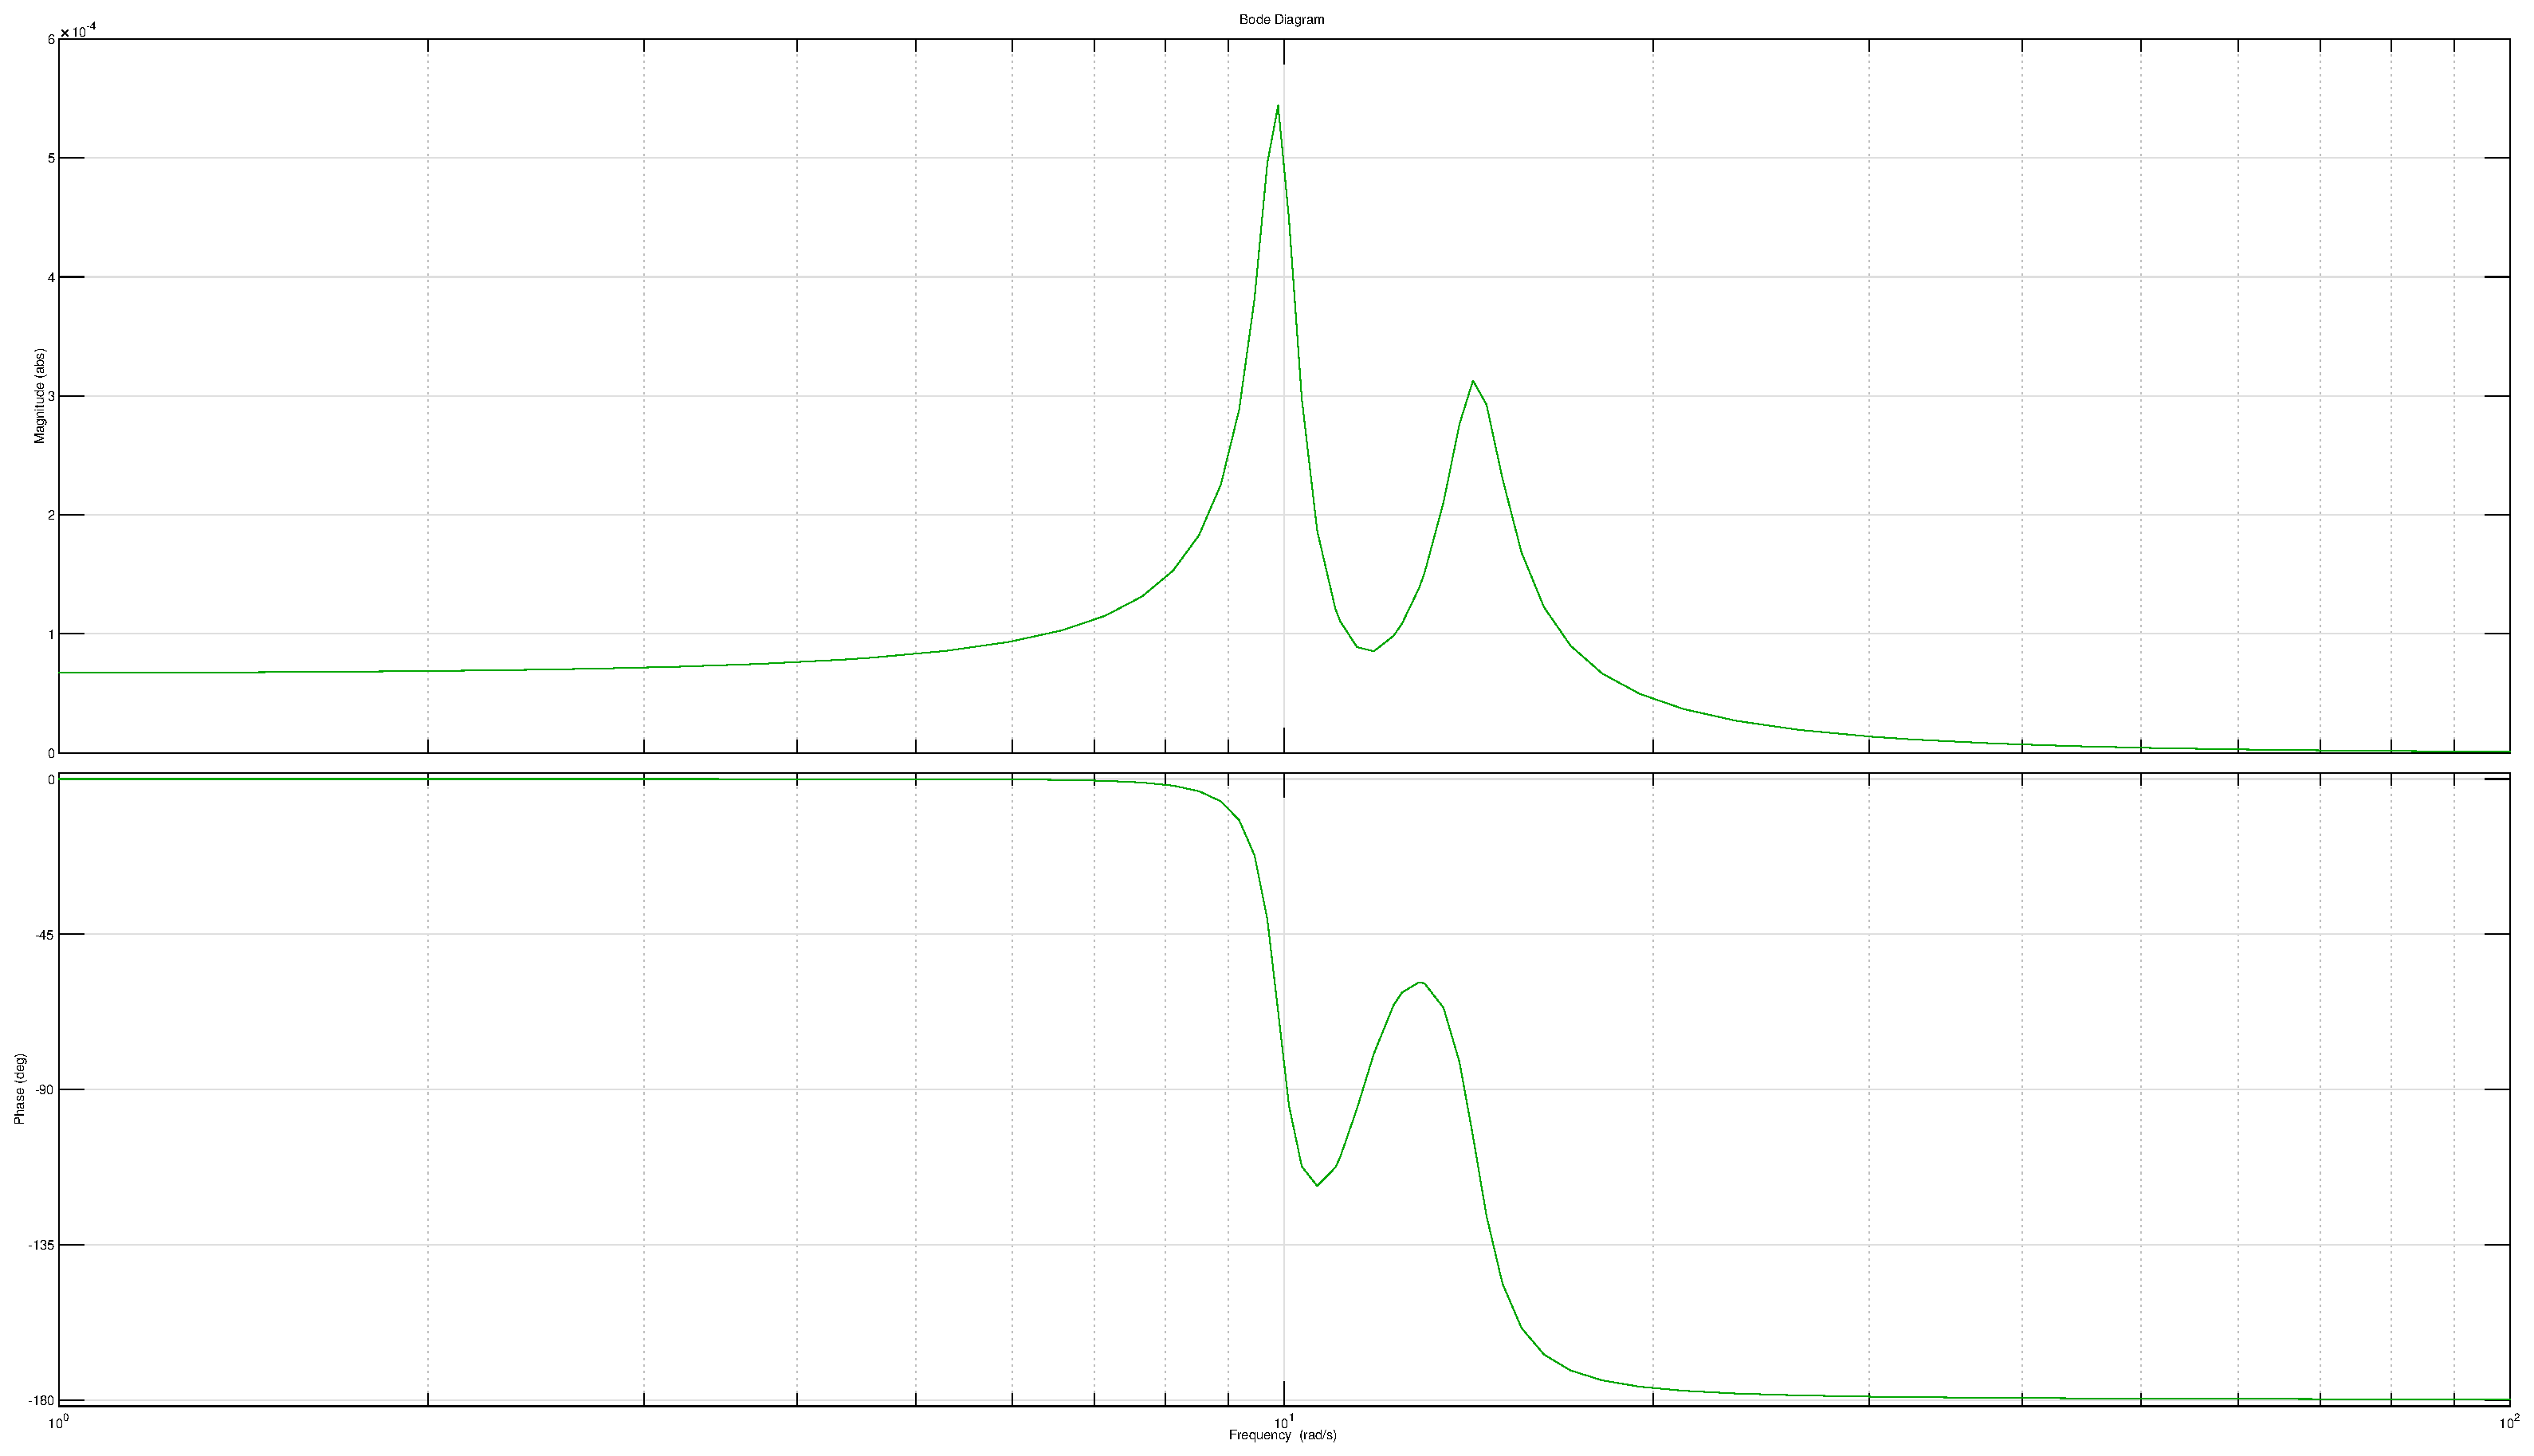
\includegraphics[width=0.75\linewidth]{bode}
	\caption{Bode diagram of tranfer matrix.}
	\label{fig:bodeplot}
\end{figure}
%
\(\mathcal{L}_{2}\) gain is a popular measure of smallness for system
approximation errors and dynamical perturbations.
Consider a causal convolution model of an LTI system, possibly of an
infinite order, defined by the impulse response matrix \(g = g(t)\) or by a
transfer matrix \(G = G(s)\).
Remember that such system defines the output \(y\) as a convolution integral.
\begin{equation}
	\label{eq:convintegral}
	y(t) = \int_{0}^{\infty} h(\tau)f(t-\tau)d\tau
\end{equation}
%
where \(f\) is assumed to vanish fast enough as \(t \rightarrow -\infty\).\\
Let \(\hat{g} = \hat{g}(t)\) and \(\hat{G} = \hat{G}(s)\) be the impulse
response and the transfer matrix of another convolution model, intended to
serve as a simplified approximation of the original one.
One common way of measuring approximation quality is by comparing system
responses \(y_{0} = y_{0}(t)\) and \(\hat{y}_{0} = \hat{y}_{0}(t)\) to a
particular ``testing" input \(f_{0} = f_{0}(t)\).
This leads to the so-called H-Infinity norm of the difference
 \(H(s) = G(s) - \hat{G}(s)\) as the approximation error measure of choice.\cite{l2gain}

	% Comunicazione
	% \input{comunicazione}
	% Modello sistema
	% \input{modellosistema}
	% \input{occgridmodel}
	% Soluzione Proposta
	% \input{soluzione}
	% Implementazione
	% \input{implementazione}
	% Risultati
	% \input{risultati}
	% Conclusioni
	% \input{conclusioni}
%-------------------------------------------------------------------------------
%	Bibliography
%-------------------------------------------------------------------------------
	\bibliographystyle{IEEEtran}
	\bibliography{bibliografia.bib}
\end{document}
